\documentclass[11pt, oneside]{article}   	% use "amsart" instead of "article" for AMSLaTeX format
\usepackage{geometry}                		% See geometry.pdf to learn the layout options. There are lots.
\geometry{letterpaper}                   		% ... or a4paper or a5paper or ... 
%\geometry{landscape}                		% Activate for for rotated page geometry
%\usepackage[parfill]{parskip}    		% Activate to begin paragraphs with an empty line rather than an indent
\usepackage{graphicx}				% Use pdf, png, jpg, or eps� with pdflatex; use eps in DVI mode
								% TeX will automatically convert eps --> pdf in pdflatex		
\usepackage{amssymb}
\usepackage{amsmath}
\usepackage{parskip}
\usepackage{color}

\title{Newton to Kepler}
%\author{The Author}
%\section{}
% \subsection*{R code}
\date{}							% Activate to display a given date or no date

\graphicspath{{/Users/telliott_admin/Dropbox/Tex/png/}}

% \begin{center} 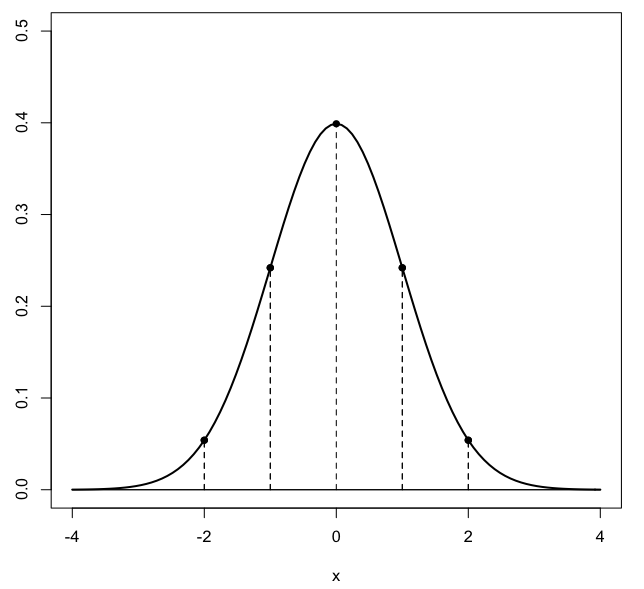
\includegraphics [scale=0.4] {gauss3.png} \end{center}

\begin{document}
\maketitle
\large
\noindent

\section{Introduction}

I'm trying to understand in detail how Kepler's Laws for the orbits of the planets can be derived from Newton's Laws ($\mathbf{F} = m \mathbf{a}$ and the inverse square law of gravitation).  I've worked through derivations from several sources, but each of them has a step that I'm not completely sure of.  My goal here is to clearly document things so that I will understand in a year or two when I re-read this.

Kepler's Laws are that first (K1) the orbits of the planets are not circles but ellipses (non-recurrent orbits may be other conic sections);  second (K2) the area or arc "swept out" per unit time is the same no matter where in the orbit the planet is;  and third (K3) the period of the orbit is independent of the mass of the planet and its square is proportional to the cube of the length of the semi-major axis of the ellipse.

\section{Kepler 2}

Kepler's second law (K2) is the easiest to prove, even without simplifying things by assuming circular orbits.  K2 states that the orbits of the planets (or other satellites) sweep out \emph{equal areas in equal times}.

\subsection*{Newton}

Here is the geometric proof used by Newton.

\begin{center} 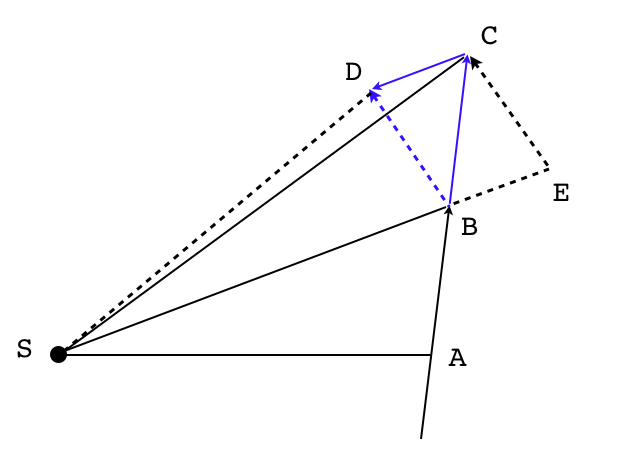
\includegraphics [scale=0.5] {newton_area.png} \end{center}

We diagram the sun $S$ and a planet at $A$.  Imagine that the force toward the sun is applied discretely.  That is, for a sufficiently small interval $\Delta t$, the planet travels from $A$ to $B$ at constant velocity and if undisturbed, would travel to $C$ in the next unit of time.  

Without any force, the velocity would be constant and so the length of $AB$ is the same as that of $BC$, and since $AB$ is on the same line as $BC$, the area of $\triangle ABS$ is equal to the area of $\triangle BCS$.  

(Proof:  draw the vertical line from $S$ to the line containing $ABC$.  The area of either triangle is one-half the length of that altitude times the distance, either $AB$ or $BC$).

Now, suppose the force is applied at $B$ \emph{toward the sun} along $EBS$.  As a result, the trajectory $BC$ is modified by the change in velocity resulting from application of the force toward the sun. The new path is the additional velocity times $\Delta t$.  Call the length $CD$ and add it to $BC$ to give the actual trajectory, $BD$.  

$CD$ is parallel to $SBE$.  Therefore, every point on $CD$ has an altitude with respect to $SBE$ of the same length.  So any point on $CD$ can be used to draw a triangle with the same base $SB$ and the result will have the equal area no matter which point is chosen.

In particular, the area of $\triangle BDS$ is equal to the area of $\triangle BCS$, which was found earlier to be equal to the area of $\triangle ABS$.  Since the two triangles from the actual motion have the same area, the area is constant.

\subsection*{Feynman}

Richard Feynman gave a famous series of talks at Cornell in 1964 that were videotaped and transcribed into a book.  Bill Gates later purchased them and put them on the web, unfortunately with some Microsoft DRM.  Still, I have the book, called \emph{The Character of Physical Law}.  This argument is from Chapter 2, \emph{The Relation of Mathematics to Physics}.

It depends on a tiny bit of calculus---specifically, the product rule for differentiation.  It also uses the fact that the product rule is valid for vector cross products.  (See my short write-up on the cross-product for a proof).

The rule is that if we have two vectors $\mathbf{a}$ and $\mathbf{b}$ which are changing (i.e. they are functions of time), then

\[ \frac{d}{dt} \ (\mathbf{a} \times \mathbf{b}) = \frac{d\mathbf{a}}{dt} \times \mathbf{b} + \mathbf{a}  \times \frac{d\mathbf{b}}{dt}    \]

In our application the two vectors are the position vector of the planet with respect to the sun, $\mathbf{r}$, and the time-derivative of that vector.

\[ \frac{d\mathbf{r}}{dt} = \mathbf{v} \]

Or, as the physicists would write it, using Newton's dot notation for the time-derivative:

\[ \mathbf{v} = \dot{\mathbf{r}} \]

We are interested in the area of the triangle formed by the vectors $\mathbf{r}$ and $\dot{\mathbf{r}}$ over a small interval of time.  The area swept out is constant, as we have seen, and will prove again in a moment.

A nice feature of the vector cross-product is that it provides (twice) this area.  Namely

\[ A =  \mathbf{r} \times \dot{\mathbf{r}} = |\mathbf{r}| |\dot{\mathbf{r}}| \sin \theta   \]

where $\theta$ is the angle between $\mathbf{r}$ and $\dot{\mathbf{r}}$, and $A$ is the little bit of additional area.  (We used $\Delta A$ for this area above, the change in notation does not affect the argument below).

Our hypothesis is that $A$ is the same no matter where the planet is in its orbit.  Another way to say the same thing is that A doesn't change with time

\[ \frac{d}{dt} \ A = \dot A = 0 \]

Now 

\[ A = \mathbf{r} \times \dot{\mathbf{r}} \]

and we want to compute $\dot A$.  Using the product rule that we had above it's easy.

\[ \dot A = \frac{d}{dt} \ (\mathbf{r} \times \dot{\mathbf{r}}) \]
\[ \dot A = \dot{\mathbf{r}} \times \dot{\mathbf{r}} \ + \ \mathbf{r} \times \ddot{\mathbf{r}} \]

As Feynman says: it's just playing with dots.

So let's look at those two terms.  Another nice fact about the cross-product is that if the two vectors point in the same direction, then the cross-product is zero.

Any vector points in the same direction as itself, so the first term is certainly zero.  

\[ \dot{\mathbf{r}} \times \dot{\mathbf{r}} \ = 0 \]

Next, recall that the second derivative with respect to time of the position is the acceleration vector.  According to Newton's second law, the force of gravity points toward the sun, radially.  

But of course the position vector also points out radially from the sun.  $\mathbf{r}$ and $\ddot{\mathbf{r}}$ are in the same direction (the opposite direction \emph{is} the same direction, multiplied by $-1$), so the cross-product is again zero.

\[ \mathbf{r} \times \ddot{\mathbf{r}} \ = 0 \]

So that means the whole thing is zero.

\[ \dot A = \dot{\mathbf{r}} \times \dot{\mathbf{r}} \ + \ \mathbf{r} \times \ddot{\mathbf{r}} = 0 + 0 = 0  \]

We have shown that the area is constant.

By the way, the invariant quantity 

\[ \mathbf{r} \times \mathbf{v} = \mathbf{r} \times \dot{\mathbf{r}} = \mathbf{L} \]

is the angular momentum, and the lack of change is the principle of the conservation of angular momentum.

\section{Ellipses}

Now, a bit about ellipses.  We will not assume this for the derivations, since we are going the other way, from Newton to Kepler.  But it might help to clarify things.

This whole problem of the orbits would be trivial if they were circular.  Then, the velocity vector $\mathbf{v} = \dot{\mathbf{r}}$ would be perpendicular to the position vector $\mathbf{r}$.  On an ellipse, that isn't true.  Newton's diagram is drawn above with $AB$ not perpendicular to $AS$.

But in an elliptical orbit, the planet's velocity is in the same direction as the tangent vector to the ellipse at that position.  And the tangent vector has a nice relationship to the radial vector.  I show this by a geometric argument in the short write-up about the parametrization of the ellipse.  However, we can get to the point more quickly by writing the parametrization

\[ x = \cos \theta = \cos \omega t \]
\[ y = \sin \theta = \sin \omega t \]
\[ \mathbf{r}(t) = \ \langle x(t),y(t) \rangle \ \]
\[ = \ \langle  \cos \omega t , \sin \omega t \rangle \]
\[ \mathbf{v} = \dot{\mathbf{r}} \]
\[ = \ \langle -\omega \sin \omega t, \omega \cos \omega t \rangle \]

(more here)

\section{Hartig}
This is a derivation of Kepler's laws from a class handout I found on the web for Math 304 by Hartig.

\subsection{}
We start by defining $M$ as the mass of the sun and $m$ as the mass of the planet and $\mathbf{r}$ as the position vector from the sun to the planet.  Combining Newton's second law and the inverse square law of gravitation we have that
 
\[ \mathbf{F} = m \mathbf{a} = -\frac{GMm}{r^2} \ \frac{\mathbf{r}}{r}  \]
\[ \mathbf{a} = -\frac{GM}{r^2} \ \frac{\mathbf{r}}{r}  \]

We take $\mathbf{u_r}$ as a unit vector in the same direction as $\mathbf{r}$.  I am writing $\hat{\mathbf{u_r}}$ without its hat ( $\hat{}$ ) as $\mathbf{u_r}$ so as not to confuse it with the derivative $\dot{\mathbf{u_r}}$.

\[ \mathbf{r} = r \mathbf{u_r} \]
\[ \mathbf{a} = -\frac{GM}{r^2} \ \mathbf{u_r}  \]

The acceleration is along the line of the radial vector, pointing toward the sun.

\subsection{}
The velocity is the time-derivative of the position vector $\mathbf{r}$.

\[ \mathbf{v} = \frac{d\mathbf{r}}{dt} = \dot{\mathbf{r}} \]

and the acceleration is

\[ \mathbf{a} = \frac{d\mathbf{v}}{dt} = \ddot{\mathbf{r}} \]

\subsection{Feynman's dots, again}
We set up the angular momentum as 

\[ \mathbf{L} = \mathbf{r} \times \mathbf{p}  =  \mathbf{r} \times m\mathbf{v}\]

For a unit mass this is

\[ \mathbf{r} \times \mathbf{v} =  \mathbf{r} \times \dot{\mathbf{r}} \]

We compute the time-derivative

\[ \frac{d}{dt} (\mathbf{r} \times \dot{\mathbf{r}}) \]

by the standard vector application of the product rule which we've looked at above, this is equal to 

\[ =  \dot{\mathbf{r}} \times \dot{\mathbf{r}} + \mathbf{r} \times \ddot{\mathbf{r}} \]

and this is equal to zero, since any vector's cross product with itself is zero, including a reversed version of itself, as in the second term.  We define a constant vector $\mathbf{c}$ such that

\[ \mathbf{c} = \mathbf{r} \times \dot{\mathbf{r}} \]

Since $\mathbf{c}$ is a constant, unchanging in both direction and magnitude, it defines a normal vector to the plane containing $\mathbf{r}$ and $\dot{\mathbf{r}}$.  Align $\mathbf{c}$ with the $z$-axis so all the motion occurs in the $xy$-plane.
Note that 

\[ c = |\mathbf{c}| = | \mathbf{r} \times \dot{\mathbf{r}} | = rv \sin \theta \]

where these are all scalar quantities and $\theta$ is the angle between $\mathbf{r}$ and $\dot{\mathbf{r}} = \mathbf{v}$.

\subsection{Equal area}
We consider the triangle formed by the position vector before and after a short period of time $\Delta t$, and the vector $\Delta \mathbf{r}$ connecting these two positions, where 

\[ \Delta \mathbf{r} \approx \dot{\mathbf{r}} \Delta t \]

The little bit of area $\Delta A$ that is swept out during this time is 

\[ \Delta A \approx \frac{1}{2} \ |\mathbf{r} \times  \dot{\mathbf{r}} \Delta t | \]
\[ \Delta A = \frac{c}{2} \ \Delta t \]

So we have that

\[ \frac{\Delta A}{\Delta t} \approx \frac{c}{2}  \]

and in the limit as $\Delta t \rightarrow 0$

\[ \frac{dA}{dt} = \frac{c}{2}  \]

(Note a difference with Feynman.  He uses $A$ for the area, but never actually computes its value $|\mathbf{r} \times \dot{\mathbf{r}}|$.  Here, $dA/dt$ is the area and it's the second derivative $d^2A/dt^2$ that is equal to zero.  Which is another way of saying that $\mathbf{c}$ is constant).

\subsection{Manipulating $\mathbf{a} \times \mathbf{c}$}
The crucial step is to prove that

\[ \mathbf{a} \times \mathbf{c} = GM \dot{\mathbf{u_r}} \]

This takes a bit of work, so I'd like to defer it until the end.  We'll just assume it for now.  Take the equality and integrate with respect to time, obtaining

\[ \int \mathbf{a} \times \mathbf{c} = \int GM \dot{\mathbf{u_r}} \]
\[ \dot{\mathbf{r}} \times \mathbf{c} = GM \mathbf{u_r} + \mathbf{d} \]

where $\mathbf{d}$ is a constant \emph{vector} of integration.

\subsection{Dot product}
We're almost there now.  Take the left-hand side from above and form the dot product

\[ \mathbf{r} \cdot (\dot{\mathbf{r}} \times \mathbf{c}) \]

Use another vector identity to switch it around

\[ = (\mathbf{r} \times \dot{\mathbf{r}}) \cdot \mathbf{c} \]

But $\mathbf{r} \times \dot{\mathbf{r}} = \mathbf{c}$ so

\[ = \mathbf{c}  \cdot \mathbf{c} = c^2 \]

\subsection{Conic section}
What we've shown is that

\[ c^2 = \mathbf{r} \cdot (GM \mathbf{u_r} + \mathbf{d} ) \]
\[ = r(GM + d \cos \theta) \]
\[ = rGM(1 + \frac{d}{GM} \cos \theta ) \]

Define $k = c^2/GM$ and $e = d/GM$.  Then

\[ k = r(1 +e\cos \theta) \]

This is the equation of a conic section.  In particular, if $ e < 1$, then

\[ r = \frac{k}{1 +e\cos \theta} \]

is the equation of an ellipse.  Here is an example with $k=1$ and $e=0.6$

\begin{center} 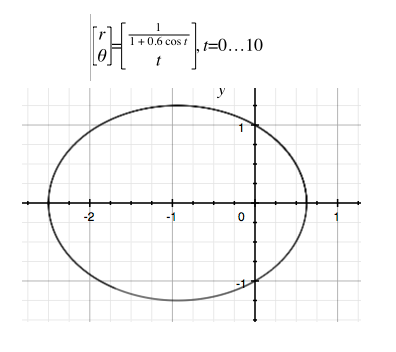
\includegraphics [scale=0.75] {ellipse_param.png} \end{center}

\subsection{Cleaning up}
Here is a sketch of the situation

\begin{center} 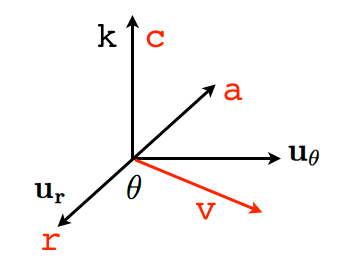
\includegraphics [scale=0.5] {Newton_vecs.png} \end{center}

As we've said all along, $\mathbf{u_r}$ is a unit vector in the $\mathbf{r}$ direction, so that $\mathbf{r} = r \mathbf{u_r}$.  By the central force hypothesis, the acceleration $\mathbf{a} = \dot{\mathbf{v}} = \ddot{\mathbf{r}}$ is in the $- \mathbf{u_r}$ direction.  The source of all our complexity is that $\mathbf{v} = \dot{\mathbf{r}}$ is not perpendicular to $\mathbf{u_r}$ but has an angle $t$ or $\theta$ with it.

Also, we defined

\[ \mathbf{c} = \mathbf{r} \times \mathbf{v} \]

and aligned $\mathbf{c}$ with the $\hat{\mathbf{k}}$ direction.  We analyzed $\mathbf{r} \times \mathbf{v}$ to show that $\mathbf{c}$ is a constant vector.

We haven't talked about $\mathbf{u_\theta}$ yet, but it is the unit vector orthogonal to $\mathbf{u_r}$.

According to Hartig, what we have to prove is that

\[ \mathbf{a} \times \mathbf{c} = GM \dot{\mathbf{u_r}} \]

Since the rest of the proof flowed so easily after this point, it seems like it must be true.  But consideration of the geometry shows an error, and I've not yet been able to reconcile the error with the rest of it.  The error is that $-\mathbf{c} \times \mathbf{a}$ is in the $\mathbf{u_\theta}$ direction, not the $\dot{\mathbf{u_r}}$ or $\mathbf{v}$ direction.

To get the whole vector, write

\[ \mathbf{r} = r \mathbf{u_r} \]
\[ \mathbf{v} = \frac{dr}{dt} \mathbf{u_r} + r \dot{\mathbf{u_r}} \]
\[ \mathbf{c} = \mathbf{r} \times \mathbf{v} = r \mathbf{u_r} \times (\frac{dr}{dt} \mathbf{u_r} + r \dot{\mathbf{u_r}}) \]

The first term is zero and the second is $r^2 \hat{\mathbf{k}}$.  Now do

\[ \mathbf{a} \times \mathbf{c} = -\frac{GM}{r^2}\mathbf{u_r} \times r^2 \hat{\mathbf{k}} = GM \mathbf{u_\theta} \]

The magnitude is correct but the direction is not.
But perhaps we can save the situation with the result from the next section!  There we will show that

\[ \dot{\mathbf{u_r}} = \frac{d \theta}{dt} \mathbf{u_\theta} \]

Call $d\theta/dt$ the angular velocity

\[ \dot{\mathbf{u_r}} = \omega \mathbf{u_\theta} \]

So, within a factor of $\omega$ we can substitute 

\[ \frac{1}{\omega} \dot{\mathbf{u_r}} = \mathbf{u_\theta} \]

and then we have

\[ \mathbf{a} \times \mathbf{c} = GM \mathbf{u_\theta} = \frac{GM}{\omega} \ \dot{\mathbf{u_r}} \]

We integrate the left-hand side easily and  $\omega$ is a constant.  So we have

\[ \mathbf{v} \times \mathbf{c} = \frac{GM}{\omega} \mathbf{u_r} \]

\section{Varberg preliminaries}

Varberg has two preliminary examples to work through (Example 14.4 and 14.5) that give results we will use in the main section of the proof.

The first example introduces $\mathbf{L}$, described as a unit vector-valued function (of time).  As they say

\[ |\mathbf{L}| = 1 \ \ \ \text{for all } t \]

$\mathbf{L}$ has unit length and it points in the same direction as $\mathbf{r}$.  That is

\[ \mathbf{r} = r \mathbf{L} \]

where $r = |\mathbf{r}|$.  At this point, for consistency, I'm going to switch back to the notation used by Hartig, where this vector is just $\mathbf{u_r}$

\[ \mathbf{r} = r \mathbf{u_r} \]

The description is that $\mathbf{u_r}$ forms an angle $\theta$ with the horizontal.  So in Cartesian coordinates

\[ \mathbf{u_r} = \langle \ \cos \theta (t), \sin \theta (t) \ \rangle \]

The result we are supposed to prove is:

\[ \frac{d}{dt} \ \mathbf{u_r} = \frac{d \theta}{dt} \ \mathbf{u_\theta} \]

where $\mathbf{u_\theta}$ is $\perp$ to $\mathbf{u_r}$ and is also a unit vector.  Furthermore, the orientation is that we must "turn left" in going from $\mathbf{u_r}$ to $\mathbf{u_\theta}$.  To find the vector $\mathbf{u_\theta}$ perpendicular or orthogonal to $\mathbf{u_r}$, we observe that

\[ \mathbf{u_r} \perp \mathbf{u_\theta} \iff \mathbf{u_r} \cdot \mathbf{u_\theta} = 0 \]

So we make a guess

\[ \mathbf{u_\theta} =  \langle \ -\sin \theta (t), \cos \theta (t) \ \rangle \]

chosen so that the dot product $\mathbf{u_r} \cdot \mathbf{u_\theta}$  is zero, and with the minus sign placed so that the direction is "to the left".  To show this, align $\mathbf{u_r}$ with $\hat{\mathbf{i}}$ and $\mathbf{u_\theta}$ with $\hat{\mathbf{j}}$, and then compute $\mathbf{u_r} \times \mathbf{u_\theta} = \langle \ 0,0,1 \ \rangle = \hat{\mathbf{k}}$.  Furthermore, $\mathbf{u_\theta}$ is of unit length.

Now just compute the derivative:

\[ \mathbf{u_r} = \langle \ \cos \theta (t), \sin \theta (t) \ \rangle \]
\[ \frac{d}{dt} \ \mathbf{u_r}= \langle \ -\sin \theta (t) \ \frac{d\theta}{dt}, \cos \theta (t) \ \frac{d\theta}{dt} \ \rangle \]
\[ = \frac{d\theta}{dt} \ \langle \ -\sin \theta (t), \cos \theta (t) \ \rangle \]
\[  \frac{d \mathbf{u_r}}{dt} = \frac{d\theta}{dt} \ \mathbf{u_\theta} \]
\[  \dot{\mathbf{u_r}} = \frac{d\theta}{dt} \ \mathbf{u_\theta} \]

The rate of change of $\mathbf{u_r}$ with time is equal to the rate of change of the angle with time, pointed in the direction perpendicular and "to the left" of $\mathbf{u_r}$.

This looks strange to me geometrically, but I can't find anything wrong with the argument.

Don't be tempted to identify $\mathbf{u_\theta}$ with $\hat{\mathbf{T}}$, the unit vector tangent to the curve, in the same direction as $d\mathbf{r}$ and the velocity $d\mathbf{r}/dt$, but the thing here is that this path is an ellipse and in particular this statement is \emph{not} true:  $\mathbf{r} \perp \mathbf{v}?$

\section{Varberg}

Now we're going to proceed with the derivation based on Varberg \emph{Calculus} (online version only, Chapter 14).

One change I feel I need to introduce is to use $\mathbf{r}$ for the position vector (following Feynman) rather than $\mathbf{X}$, as Varberg do, in addition to the substitution of $\mathbf{u_r}$ and $\mathbf{u_\theta}$ we did above.

\subsection*{Example 14.5}

The second example relates to the following diagram

\begin{center} 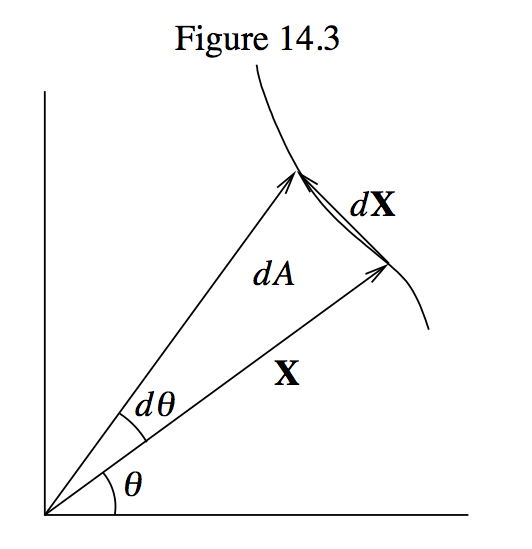
\includegraphics [scale=0.4] {Varberg14_3.png} \end{center}

As mentioned before, the problem uses $\mathbf{X}$ for the position vector, but I will label it as $\mathbf{r}$, following Feynman.  This vector "stays always in the $xy$-plane."  Also, as above, I will use $\mathbf{u_r}$ for the vector they call $\mathbf{L}$ and similarly $\mathbf{u_\theta}$ for the vector they call $\mathbf{L}^{\perp}$.

We are asked to show that

\[ \frac{dA}{dt} = \frac{1}{2} \ | \frac{d\mathbf{r}}{dt} \times \mathbf{r} | \]

This presentation is a bit different than Feynman's, and it confused me for a while, because, just for starters, we proved before that $dA/dt = 0$ but that will not be the case here, because now $dA/dt$ means something different.

What I'm going to do is to say that in a short time $\Delta t$, the area that is swept out is $\Delta A$, corresponding to a length $d\mathbf{r} = \mathbf{v} \Delta t$, and that by the geometry we have

\[ 2 \Delta A = |\mathbf{r} \times \mathbf{v} \Delta t | \]

I assert that it is OK to bring $\Delta t$ out of the cross product, since it is a constant at any one stage of its future journey to the limit $\Delta t \rightarrow 0$, so I write

\[ 2 \Delta A = |\mathbf{r} \times \mathbf{v} | \Delta t \]

Now we have 

\[ 2 \frac{\Delta A}{\Delta t} = |\mathbf{r} \times \mathbf{v} | \]

and in the limit

\[ 2 \frac{dA}{dt} = |\mathbf{r} \times \mathbf{v} | \]

Now this is almost what we were asked to prove, but recall that

\[ \frac{d\mathbf{r}}{dt} \times \mathbf{r} = \dot{\mathbf{r}}  \times \mathbf{r} = - \mathbf{r} \times \dot{\mathbf{r}} \]

so the absolute values are the same.  Again, the result is that

\[ 2\frac{dA}{dt} =  | \dot{\mathbf{r}} \times \mathbf{r} | = | \mathbf{r} \times \dot{\mathbf{r}} | \]


Varberg \emph{et al.} give a second argument which goes as follows.  By the geometry of the triangle, the area is

\[ 2 \ dA = r \ r d \theta = r^2 d \theta \]

where $r$ is $|\mathbf{r}|$.  And then they say

\[ 2 \ \frac{dA}{dt} = r^2 \ \frac{d\theta}{dt}  \]

They do this without comment, but this result assumes that $r$ does not vary with time, although clearly it does (that's the whole point).  The product rule would give us:

\[ \frac{d}{dt} \ r^2 d \theta = 2 r \ d \theta  \ \frac{dr}{dt} + r^2 \ \frac{d\theta}{dt}  \]

This looks a little weird because of the single differential $d\theta$, but I think what it means is that in the limit, the first term goes to zero.

Another way of explaining this is to break the area into two parts.  The first part is $(1/2) r$ times $r \ d\theta$, the length of (almost straight) arc perpendicular to $\mathbf{r}$.  This is the part we get by assuming that $r$ is constant.  And in the limit as $t \rightarrow 0$, the resulting $d\theta/dt$ has some value, namely, the angular velocity.

The second part is $(1/2) r \ d\theta$ times $dr$.  This is the part that accounts for the change in $r$, but it contains two differentials, only one of which gets rescued into some quantity by $dt$.  The other just goes to zero, so the whole thing is zero. 

Anyway, let's continue with the argument.

Go back to the right-hand side of what we were asked to prove above

\[ 2 \ \frac{dA}{dt} =  | \frac{d\mathbf{r}}{dt} \times \mathbf{r} | \]

and show that it turns into $r^2 d\theta/dt$.  Using $\mathbf{u_r}$ for the unit vector in the $\mathbf{r}$ direction, we have

\[ \frac{d\mathbf{r}}{dt}  = \frac{d}{dt} (r \mathbf{u_r}) = \frac{dr}{dt} \mathbf{u_r} + r \frac{d\mathbf{u_r} }{dt}  \]

where the first part is just separating the scalar and unit vector part of $\mathbf{r}$ and the rest is from the product rule.  At this point we recall the result from the first example (that $d \mathbf{u_r}/dt  = d \theta/dt \ \mathbf{u_\theta}$), so we have

\[ = \frac{dr}{dt} \mathbf{u_r} + r  \frac{d \theta}{dt} \ \mathbf{u_\theta} \]

So now this is what we need to cross with $\mathbf{r}$, also known as $r \mathbf{u_r}$.  We write

\[ (\frac{dr}{dt}  \mathbf{u_r} + r  \frac{d \theta}{dt} \  \mathbf{u_\theta}) \times r  \mathbf{u_r} \]
\[ = (\frac{dr}{dt}  \mathbf{u_r} \times  r  \mathbf{u_r}) + (r  \frac{d \theta}{dt} \  \mathbf{u_\theta} \times r  \mathbf{u_r}) \]

The first term is zero, and because these are unit vectors the absolute value of the second term's vector cross-product is $1$

\[ | r  \frac{d \theta}{dt} \ \mathbf{u_\theta} \times r \mathbf{u_r} | = r^2 \frac{d \theta}{dt} \]

So what we've shown is that 

\[ 2 \ \frac{dA}{dt} =  | \mathbf{r} \times \dot{\mathbf{r}} | \]

and

\[ 2 \ \frac{dA}{dt} =  r^2 \ \frac{d \theta}{dt} \]

This term ($r^2 d\theta/dt$) is what Hartig calls $c$.  It points in the $\hat{\mathbf{k}}$ direction and is just the angular momentum without the mass component, and it is what Varberg will call $\mathbf{H}$, below.

\subsection*{Kepler's Second Law K2}

K2 says that orbits "sweep out equal areas in equal times" or equivalently, that $dA/dt = 0$.  So we start from Newton's force directed toward the sun, the centripetal force, and we will show that the motion stays in a plane, and also implies K2.

Again, this is Feynman's argument (and notation)

\[ \frac{d}{dt} ( \mathbf{r} \times \mathbf{v}) = \frac{d}{dt} ( \mathbf{r} \times \dot{\mathbf{r}}) = 0 \]

This is zero because you get two terms from the derivative of the cross-product:  one is $\dot{\mathbf{r}} \times \dot{\mathbf{r}} = 0$ , and the second one is $\mathbf{r} \times \ddot{\mathbf{r}}$, which is zero because these two vectors point in opposite directions by the centripetal force postulate.

Therefore,  $\mathbf{r} \times \dot{\mathbf{r}}$ is constant.  We will say that

\[ \mathbf{r} \times \dot{\mathbf{r}} = \mathbf{H} \]

and 

\[ |\mathbf{H}| = h = 2 \ \frac{dA}{dt} \]

If $\mathbf{H} = 0$, there is no force, and just straight-line motion.  But for  $\mathbf{H} \ne 0$, then $\mathbf{r}$ and $\dot{\mathbf{r}}$ are in a plane that doesn't change with time, and $\mathbf{H}$ is the normal vector of that plane.

\[ h = | \mathbf{r} \times \dot{\mathbf{r}} | = |\mathbf{r} \times \frac{d\mathbf{r}}{dt} | \]

by the example above ($14.5$)

\[ h =  r^2 \ \frac{d \theta}{dt} = 2 \ \frac{dA}{dt} \]

This is the statement of K2.  $dA/dt$ is constant, equal to $h/2$.

\subsection*{reverse}

Now we are going to reverse the argument and show that planar motion and K2 imply a centripetal force.  Planar motion means that $\mathbf{r} \times \dot{\mathbf{r}}$ has fixed direction (again, normal to the plane), and K2 means that it has constant magnitude.  Since it doesn't change with time

\[ \frac{d}{dt} (\mathbf{r} \times \dot{\mathbf{r}}) = 0 \]

but 

\[ \frac{d}{dt} (\mathbf{r} \times \dot{\mathbf{r}}) = \dot{\mathbf{r}} \times \dot{\mathbf{r}} + \mathbf{r} \times \ddot{\mathbf{r}}  \]

Now $\dot{\mathbf{r}} \times \dot{\mathbf{r}}$ is always zero, so that means the second term

\[ \mathbf{r} \times \ddot{\mathbf{r}} = \mathbf{r} \times \mathbf{a} = 0 \]

The acceleration vector $\mathbf{a}$ is parallel to the position vector.

\subsection*{Kepler's First Law K1}

We make an additional hypothesis due to Newton, which is that the acceleration is proportional to the inverse square of the distance from the sun (origin), and pointed toward it.

\[ \mathbf{a} = \ddot{\mathbf{r}} = - \frac{k}{r^2} \mathbf{u_r} \]

where $\mathbf{u_r}$ is the \emph{unit} vector in the $\mathbf{r}$ direction (i.e. equal to $\mathbf{r}/|\mathbf{r}|$), and $k$ is a constant (namely $GM$), not to be confused with the unit vector $\hat{\mathbf{k}}$.

The first of three main steps in the proof is to take the cross-product with $\hat{\mathbf{k}}$ (as the text says, "this allows us to introduce the area information in vectorial form")

\[ \ddot{\mathbf{r}} \times \hat{\mathbf{k}} = - \frac{k}{r^2} \ \mathbf{u_r} \times \hat{\mathbf{k}} = \frac{k}{r^2} \ \mathbf{u_\theta} \]

(recall that we "go to the left" for $\mathbf{u_\theta}$).  It should not be surprising that the cross-product brings us back to $\mathbf{u_\theta}$.  We aligned $\mathbf{u_r} \times \mathbf{u_{\theta}}$ with $\hat{\mathbf{k}}$.

For any three orthogonal vectors (say the standard vectors), if

\[ \hat{\mathbf{i}} \times \hat{\mathbf{j}} = \hat{\mathbf{k}} \]

then

\[ \hat{\mathbf{j}} \times \hat{\mathbf{k}} = \hat{\mathbf{i}} \]
\[ \hat{\mathbf{k}} \times \hat{\mathbf{i}} = \hat{\mathbf{j}} \]

By example 14.4 above

\[ \frac{d \mathbf{u_r}}{dt}= \frac{d\theta}{dt} \ \mathbf{u_\theta} \]
\[ \mathbf{u_\theta} = \frac{d \mathbf{u_r}/dt}{d\theta/dt } \]

and from K2

\[ \frac{d \theta}{dt} = \frac{h}{r^2} \]

Hence

\[  \mathbf{u_\theta} = \frac{d \mathbf{u_r}/dt}{d \theta / dt} = \frac{d \mathbf{u_r}/dt}{h/r^2} \]

So the cross-product

\[ \ddot{\mathbf{r}} \times \hat{\mathbf{k}} = \frac{k}{r^2} \  \mathbf{u_\theta} = \frac{k}{h} \ \frac{d  \mathbf{u_r}}{dt}  \]

The second clever thing we do here is to integrate with respect to time (remember that $k$, $h$ and $\hat{\mathbf{k}}$ are all constant)

\[ \dot{\mathbf{r}} \times \hat{\mathbf{k}} = \frac{k}{h} \ ( \mathbf{u_r} + \mathbf{E}) \]

where $ \mathbf{E}$ is a constant (vector) of integration.

The third step is to dot both sides with $\mathbf{r}$

\[ \mathbf{r} \cdot ( \dot{\mathbf{r}} \times \hat{\mathbf{k}}) = \frac{k}{h} \ \mathbf{r} \cdot ( \mathbf{u_r} + \mathbf{E}) \]

using the following vector identity, the left-hand side is

\[ \mathbf{r} \cdot ( \dot{\mathbf{r}} \times \hat{\mathbf{k}}) = (\mathbf{r} \times \dot{\mathbf{r}}) \cdot \hat{\mathbf{k}} \]

but 

\[ \mathbf{r} \times \dot{\mathbf{r}} = h \ \hat{\mathbf{k}} \]

so we have

\[ h \ \hat{\mathbf{k}} \cdot \hat{\mathbf{k}} = h \]

Putting it all together

\[ \mathbf{r} \cdot (\ddot{\mathbf{r}} \times \hat{\mathbf{k}}) = h = \frac{k}{h} \ \mathbf{r} \cdot ( \mathbf{u_r} + \mathbf{E}) \]

\[ \frac{h^2}{k} =  \mathbf{r} \cdot ( \mathbf{u_r}+ \mathbf{E}) \]

Recall that $ \mathbf{u_r}$ is the unit vector in the same direction as $\mathbf{r}$ so that $\mathbf{r} \cdot  \mathbf{u_r} = r$.

We can take $\mathbf{E}$ to be in the direction of $\mathbf{r}$ at time-zero so $\mathbf{r} \cdot \mathbf{E}$ is equal to $r$ times $e$ times the cosine of the angle between them at some later time.  (Since $\mathbf{E}$ is a constant vector of integration, its magnitude $e$ can be anything we want).

Thus, in polar coordinates this becomes 

\[ r(1 + e \cos \theta) = \frac{h^2}{k} \]

These curves are conic sections.  If $e < 1$ it's an ellipse.

\begin{center} 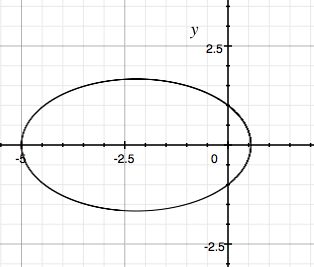
\includegraphics [scale=0.6] {quick_ellipse.png} \end{center}

The outer curve above is an ellipse with the formula

\[ r(1 + 0.1 \cos \theta) = 2 \]

(the inner is just a circle in the template that I couldn't get rid of).

$e$ is the eccentricity of the ellipse

\[ e^2 +  \frac{b^2}{a^2} = 1 \]

\subsection*{Kepler's Third Law}

The last part of Varberg's derivation is about K3.  To prove:

\[ T^2 = \frac{(2 \pi)^2}{k} \ a^3 \]

where $T$ is the period, $k$ is our constant from before, and $a$ is the length of the half-major axis of the ellipse.  In other words, the period of an orbit is the $3/2$ power of the "radius", technically the semi-major axis of the ellipse.

Start with K2

\[ 2 \ \frac{dA}{dt} =  h \]

Integrate with respect to time over one revolution obtaining an ellipse with area $\pi a b$ and the period $T$ for the time

\[ 2 \pi a b = hT \]
\[ T^2 = (\frac{2 \pi a b}{h})^2 \]

Now, go back to the equation for the orbit

\[ r(1 + e \cos \theta) = \frac{h^2}{k} \]

Consider one-half an orbit between $\theta = 0 \rightarrow \theta = \pi$.  The length of the axis is $2a$, equal to $2r$ for this orbit, so

\[ 2a = \frac{h^2}{k(1 + e \cos \pi)} +  \frac{h^2}{k(1 + e \cos 0)} \]
\[ = \frac{h^2}{k} (\frac{1}{1 - e} +  \frac{1}{1 + e}) \]
\[ = \frac{h^2}{k} \ \frac{2}{1 - e^2} \]

So

\[ a = \frac{h^2}{k} \ \frac{1}{1 - e^2} \]

For an ellipse

\[ \frac{b^2}{a^2} = 1 - e^2 \]

so
\[ a = \frac{h^2}{k} \ \frac{a^2}{b^2} \]

\[  b^2 = \frac{ah^2}{k}  \]

We had 

\[ T^2 = (\frac{2 \pi a b}{h})^2 \]
\[ = (\frac{2 \pi a }{h})^2 \  \frac{ah^2}{k}  \]
\[ = \frac{(2 \pi)^2}{k} a^3 \]

which is K3.  Recall that $k$ is $GM$, the gravitational constant times the mass of the sun.  The angular momentum $h$ has dropped out.  In other words, the period for a particular orbit does not depend on the mass of the planet or satellite.

\section{Bressoud}

Finally, I worked through a derivation of Kepler's laws from the Calculus text by Bressoud.  I'm not going to show all of it, but it starts with a more rigorous derivation of the invariant quantity as $r^2 d\theta/dt$, and also gives expressions for the velocity and acceleration in terms of  $\mathbf{u_r}$ and  $\mathbf{u_{\theta}}$.

We start with $\mathbf{u_r}$, which is the unit vector in the same direction as the position vector $\mathbf{r}$, pointing from the sun to the planet.  (We leave off the hat ( $\hat{}$ ).

\[ \mathbf{r} = r \mathbf{u_r} \]

We can write 

\[ \mathbf{r} = \ \langle r \cos \theta, r \sin \theta \rangle \]
\[ \mathbf{u_r} = \ \langle \cos \theta, \sin \theta \rangle \]

and designate the orthogonal vector

\[ \mathbf{u_{\theta}} = \ \langle -\sin \theta, \cos \theta \rangle \]

Calculate the time-derivatives

\[ \dot{\mathbf{u_r}} = \ \langle -\sin \theta \ \frac{d\theta}{dt}, \cos \theta  \ \frac{d\theta}{dt} \rangle =  \frac{d\theta}{dt} \ \mathbf{u_{\theta}} \]

\[ \dot{\mathbf{u_{\theta}}} = \ \langle -\cos \theta \ \frac{d\theta}{dt}, -\sin \theta  \ \frac{d\theta}{dt} \rangle =  -\frac{d\theta}{dt} \ \mathbf{u_r} \]

The velocity is

\[ \mathbf{v} = \frac{d}{dt} \  \mathbf{r} = \frac{d}{dt} \ r \mathbf{u_r} \]
\[ =  \frac{dr}{dt} \ \mathbf{u_r} + r \dot{\mathbf{u_r}}  \]
\[ =  \frac{dr}{dt} \ \mathbf{u_r} + r \frac{d\theta}{dt} \ \mathbf{u_{\theta}}  \]

The acceleration is

\[ \mathbf{a} = \frac{d}{dt} \  \mathbf{v} \]
\[ = \frac{d}{dt} \ (\frac{dr}{dt} \  \mathbf{u_r} + r \frac{d\theta}{dt} \ \mathbf{u_{\theta}})  \]

\[ = \frac{d^2r}{dt^2} \  \mathbf{u_r} +  \frac{dr}{dt} \frac{d\theta}{dt} \ \mathbf{u_{\theta}}  + \frac{dr}{dt} \ \frac{d\theta}{dt} \ \mathbf{u_{\theta}} + r  \frac{d^2\theta}{dt^2}  \ \mathbf{u_{\theta}}  - r (\frac{d\theta}{dt})^2 \ \mathbf{u_r} \]

Cleverly notice that 

\[ \frac{d}{dt} \ (r^2 \frac{d\theta}{dt}) = 2 r \frac{dr}{dt} \frac{d \theta}{dt} + r^2 \frac{d^2 \theta}{dt^2} \]
\[ = \frac{1}{r} (2 \ \frac{dr}{dt} \frac{d \theta}{dt} + r \frac{d^2 \theta}{dt^2}) \]

which is the same as the grouped coefficients of $\mathbf{u_{\theta}}$ from the line above.  Recognize that the only way the acceleration can be strictly radial is if these coefficients equal zero, so:

\[ \frac{d}{dt} \ (r^2 \frac{d\theta}{dt}) = 0 \]

This means that $r^2 d\theta/dt$ is a constant.

This is a lot uglier than Feynman's dots, but perhaps the expression for $\mathbf{v}$ will come in handy.


\end{document}  